\documentclass{article}

\usepackage{amssymb,amsmath,amsthm,mathtools,cancel}
\usepackage{tikz}
\usepackage[margin=1in]{geometry}
\usepackage{enumitem}

\newtheorem{theorem}{Theorem}[section]
\newtheorem{lemma}[theorem]{Lemma}

\begin{document}
\noindent
\begin{minipage}[t]{0.68\textwidth}
{\large 6.1200 \textit{Mathematics for Computer Science}}\\[4pt]
{\large Problem Set 2}\\[4pt]
{\large Solutions by Harsh Bhalala}
\end{minipage}%
\hfill
\begin{minipage}[t]{0.27\textwidth}
\raggedleft
{\large 2, October 2026}
\end{minipage}

\vspace{6pt}

\noindent\rule{\textwidth}{0.5pt}

\section*{Problem 1. Tree's Degrees}
\textbf{(a)}
\begin{proof}
Let $P(n)$ be the proposition that any tree with $n \ge 2$ vertices and $k$ vertices of degree $\ge 3$ has at least $k + 2$ leaves.

\textbf{Base Case:} $n = 2$; then $k$ must be 0, so there are at most $0 + 2$ leaves. The base case holds.

\textbf{Inductive step:} Assume $P(n-1)$ is true for $n > 2$.

Consider a tree $T$ with $n > 2$ vertices, of which $k$ have degree at least 3. Let $T' = T - l$, where $l$ is a leaf of $T$. Consider cases based on the leaf count of $T'$.
\begin{itemize}
\item \textbf{Case I:} If $l$'s parent had more than one child, the leaf count decreases by 1.
This implies the parent has degree $\geq 3$, so $|L'| = |L| - 1$ and $k' = k - 1$.
\item \textbf{Case II:} If $l$'s parent had only one child, the leaf count doesn't change.
This implies the parent has degree exactly 2, so $|L'| = |L|$ and $k' = k$.

\end{itemize}
Now Induction hypothesis on $T'$ we get $|L'| \geq k' + 2$ and now adding vertex $l$ back and substituting
value $|L'|$ and $k'$ From case I we get $|L| \geq k + 2$ ans case II also results in same equation.
Thus, by The Induction principle, $P(n)$ holds for all $n \geq 2$.

\end{proof}

\vspace{\baselineskip}
\noindent\textbf{(b)}
\begin{proof}
By the property of trees, the total number of edges $|E| = n - 1$. Now, substituting it into
Handshake Lemma yields $\sum deg(v) = 2n - 2$.

Let $l$ be the number of leaves of a tree, also k is vertices of degree at least 3, and let $n - l - k$ be the number of vertices of degree 2.
so total degree of a tree,
\[
\begin{aligned}
\sum deg(v) &\geq l + 2(n - l - k) + 3k\\
2n - 2 &\geq l + 2n - 2l -2k + 3k\\
l &\geq k + 2\\
\end{aligned}
\]
\end{proof}


\section*{Problem 2. Froli-King}
\textbf{(a)}
By modeling the chessboard as a graph where nodes represent squares of the chessboard, and there exists an edge between two
node if they are adjacent.
Now a move for the king is legal if two squares are adjacent to each other, and the total number of legal king moves is 420
and In our graph model, every legal move counts each edge twice because moves $a \rightarrow b$ and $b \rightarrow a$ are
Considered distinct moves, so the total number of edges in our graph $|E| = 420/2 = 210$

Frolicsome corresponds to an Euler tour because the graph model (a) says we must start and end at the same vertex, and (b) and (c)
implies we must visit every edge exactly once. Also, since our graph has exactly 210 edges and a move corresponds to
an edge, Frolicsome of 210 moves is just an Euler tour.

And we know an Euler tour is only possible iff every vertex is connected and has even degree. But the corner nodes have
degree of 3, which is odd.

\vspace{\baselineskip}
\noindent\textbf{(b)}

To make our graph Eulerian, we must make every vertex of even degree, and from part(a) there are a total of 28 corner
vertices with odd degree, and since they are connected, we can remove one edge between two odd-degree vertices
to make them even degree, so the total number of edges we must remove is $28 / 2 = 14$ and
if we remove corner edges alternatively, it will result in a graph with a total of
196 edges; also, each vertex is connected and has even degree.

\textbf{Corollary:} There exists a Frolicsome sequence of 196 King moves on this $8\times8$ board

\section*{Problem 3. DAGs}

\vspace{\baselineskip}
\noindent\textbf{(a)} The largest chain is (1, 2, 3, 6, 9, 10, 12).

\vspace{\baselineskip}
\noindent\textbf{(b)} The largest anti-chain is (1,4,5,7,8,11) because the remaining nodes form a chain as shown in part (a), and every element of the anti-chain is incomparable to the remaining elements.
Therefore, it's the largest possible anti-chain.

\vspace{\baselineskip}
\noindent\textbf{(c)} 12 second

\vspace{\baselineskip}
\noindent\textbf{(d)} 7 second

\vspace{\baselineskip}
\noindent\textbf{(e)} 3 processors.

\textbf{(e) Minimum Processors and Schedule}

The smallest number of processors is $p = 3$.

\vspace{1em}
\textbf{Optimal Schedule:}

\begin{center}
\begin{tabular}{|c|c|c|c|}
\hline
\textbf{Time Step} & \textbf{Processor 1} & \textbf{Processor 2} & \textbf{Processor 3} \\ \hline
$t = 1$ & 1 & 7 & 8 \\ \hline
$t = 2$ & 2 & 4 & 5 \\ \hline
$t = 3$ & 3 & 11 & \textit{Idle} \\ \hline
$t = 4$ & 6 & \textit{Idle} & \textit{Idle} \\ \hline
$t = 5$ & 9 & \textit{Idle} & \textit{Idle} \\ \hline
$t = 6$ & 10 & \textit{Idle} & \textit{Idle} \\ \hline
$t = 7$ & 12 & \textit{Idle} & \textit{Idle} \\ \hline
\end{tabular}
\end{center}

\vspace{1em}

\textbf{Proof that $2$ processors take longer:} For processors to do task 6 on t = 4, 7 tasks must be done in 3 seconds
with two processors maximum task can be done in 3 seconds = 3 $\times$ 2 = 6 which is less then 7. so p-1 or less processors will take longer than
Optimal time.

\vspace{\baselineskip}
\noindent\textbf{(f)} (1, 7, 8, 11, 4, 5, 2, 3, 6, 9, 10, 12)

\section*{Problem 4. Pok\'emon Constraints}

\textbf{(a)}
\[\phi_2 \coloneq \left( \bar{A} \lor \bar{D} \right) \left( \bar{B} \lor \bar{E} \right) \land \left( \bar{C} \lor \bar{F} \right) \land
\left( \bar{C} \lor \bar{G} \right) \land \left( \bar{F} \lor \bar{G} \right)\]

\pagebreak
\vspace{\baselineskip}
\noindent\textbf{(b)}
\begin{center}
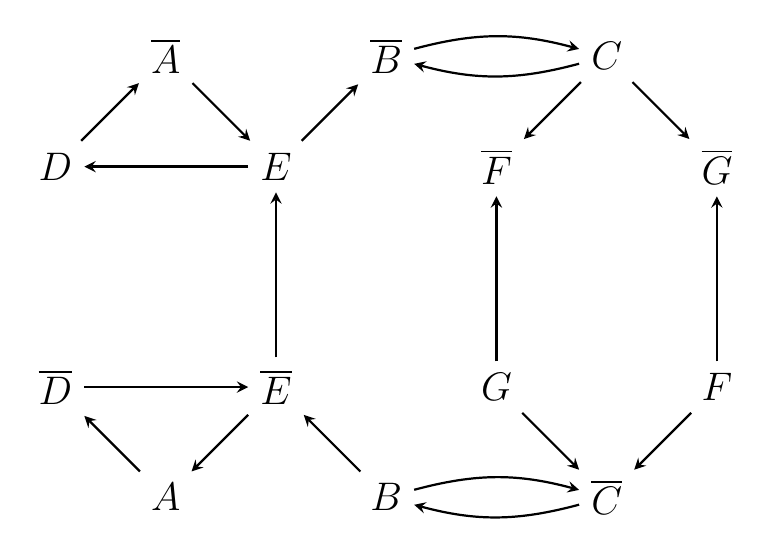
\begin{tikzpicture}[
x=1.4cm, y=1.4cm, % Uniform scale for perfect symmetry
>=stealth,
thick,
every node/.style={font=\Large, inner sep=4pt}
]

% ================= Nodes =================
% The grid is now perfectly spaced: horizontal gaps match vertical gaps
% to ensure all diagonal lines sit at exact 45-degree angles.

% Top row (y=3)
\node (Abar) at (1, 3) {$\overline{A}$};
\node (Bbar) at (3, 3) {$\overline{B}$};
\node (C) at (5, 3) {$C$};

% Upper Middle row (y=2)
\node (D) at (0, 2) {$D$};
\node (E) at (2, 2) {$E$};
\node (Fbar) at (4, 2) {$\overline{F}$};
\node (Gbar) at (6, 2) {$\overline{G}$};

% Lower Middle row (y=0) - Shifted down to create a perfect square for F/G
\node (Dbar) at (0, 0) {$\overline{D}$};
\node (Ebar) at (2, 0) {$\overline{E}$};
\node (G) at (4, 0) {$G$};
\node (F) at (6, 0) {$F$};

% Bottom row (y=-1) - Shifted down to mirror the top row's spacing
\node (A) at (1, -1) {$A$};
\node (B) at (3, -1) {$B$};
\node (Cbar) at (5, -1) {$\overline{C}$};

% ================= Edges =================

% Left block (D, \overline{A}, E)
\draw[->] (D) -- (Abar);
\draw[->] (Abar) -- (E);
\draw[->] (E) -- (D);

% Left block symmetric (A, \overline{D}, \overline{E})
\draw[->] (A) -- (Dbar);
\draw[->] (Dbar) -- (Ebar);
\draw[->] (Ebar) -- (A);

% Center Vertical self-implications (E <-> \overline{E})
\draw[->, left=15] (Ebar) to (E);

% Center Diagonal Connections crossing to the B block
\draw[->] (E) -- (Bbar);
\draw[->] (B) -- (Ebar);

% Top right cycle (\overline{B} <-> C)
\draw[->, bend left=15] (Bbar) to (C);
\draw[->, bend left=15] (C) to (Bbar);

% Bottom right cycle (B <-> \overline{C})
\draw[->, bend left=15] (B) to (Cbar);
\draw[->, bend left=15] (Cbar) to (B);

% Far Right Block Connections (C to F/G)
\draw[->] (C) -- (Fbar);
\draw[->] (C) -- (Gbar);

% Far Right Block Connections (F/G to \overline{C})
\draw[->] (F) -- (Cbar);
\draw[->] (G) -- (Cbar);

% Far Right Block Internal Edges
\draw[->] (G) -- (Fbar);
\draw[->] (F) -- (Gbar);

\end{tikzpicture}
\end{center}

\vspace{\baselineskip}
\noindent\textbf{(c)}
$P(k)$ $\coloneq$ For any arbitrary literals $x$ and $y$, if $\psi$ is true and implication graph of $\psi$ contains path $\pi$ of length $k$ from
$x$ to $y$ then $x \implies y$.
\begin{proof}[proof by Induction]
Let $\psi$ be 2-CNF formula, and let $y$, $x$ be literals in $\psi$. now assume $\psi$ is true and the implication graph of $\psi$ contains a path of lenth $k$ from $x$ to $y$.

\textbf{Base Case} (k = 1): Path of lenth 1 from $x$ to $y$ implies there is an edge directly between $x$ and $y$ and by the
definition of an edge in the implication graph, $x \implies y$.

\textbf{Inductive step:} Suppose for $P(k-1)$ is true for all $k > 1$. Now a path of length k from $x$ to $y$ can be shown as
\[x = v_0 \rightarrow v_1 \rightarrow v_2 \dots \rightarrow v_{k-1} \rightarrow v_k = y \]
Since the path from $x$ to $v_{k-1}$ is of length $k-1$, by the induction hypothesis we know $x \implies v_{k-1}$, and by the definition of an edge in the given graph, 
$v_{k-1} \implies y$. Therefore, by the transitive property of implication $x \implies y$.

So by induction hypothesis $P(k)$ is true for all $k > 0$.

\end{proof}

\vspace{\baselineskip}
\noindent\textbf{(d)}

\begin{center}
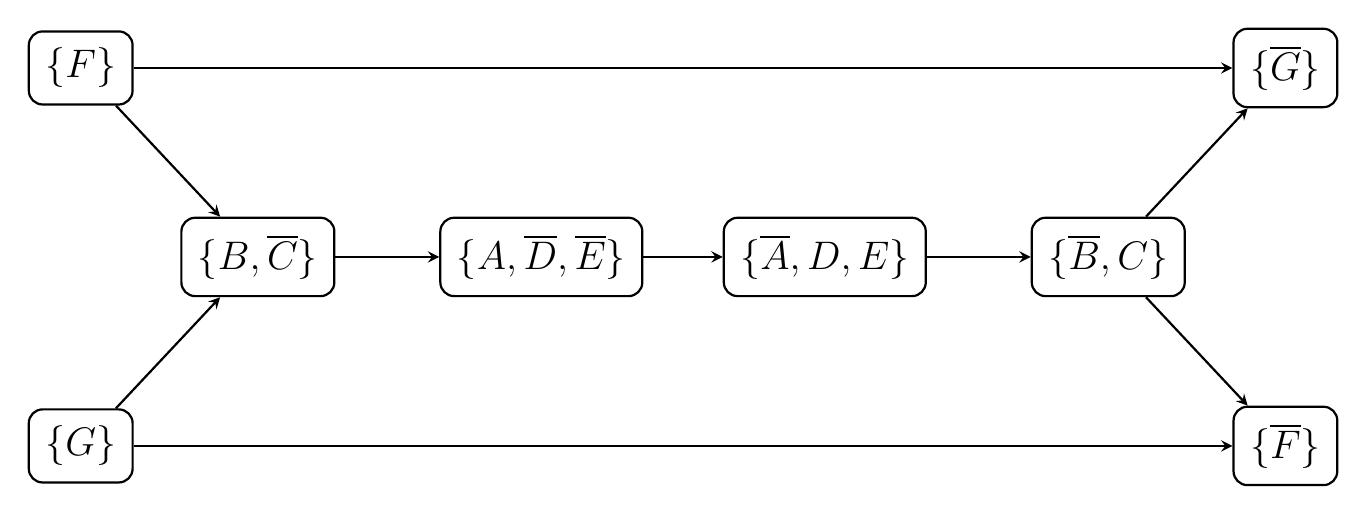
\begin{tikzpicture}[
x=0.9cm, y=1.2cm, % Scaled to fit perfectly within standard page margins
>=stealth,
thick,
every node/.style={draw, rounded corners=5pt, font=\Large, inner sep=6pt}
]

% ================= Nodes (Strongly Connected Components) =================

% Sources (Far Left)
\node (F) at (0, 2) {$\{F\}$};
\node (G) at (0, -2) {$\{G\}$};

% Central Spine (Middle)
\node (C3) at (2.5, 0) {$\{B, \overline{C}\}$};
\node (C1) at (6.5, 0) {$\{A, \overline{D}, \overline{E}\}$};
\node (C2) at (10.5, 0) {$\{\overline{A}, D, E\}$};
\node (C4) at (14.5, 0) {$\{\overline{B}, C\}$};

% Sinks (Far Right)
\node (Gbar) at (17, 2) {$\{\overline{G}\}$};
\node (Fbar) at (17, -2) {$\{\overline{F}\}$};

% ================= Edges (Between SCCs) =================

% Framing horizontal edges straight from sources to sinks
\draw[->] (F) -- (Gbar);
\draw[->] (G) -- (Fbar);

% From sources feeding into the start of the spine
\draw[->] (F) -- (C3);
\draw[->] (G) -- (C3);

% Core logical chain along the spine
\draw[->] (C3) -- (C1);
\draw[->] (C1) -- (C2);
\draw[->] (C2) -- (C4);

% From the end of the spine dispersing to the sinks
\draw[->] (C4) -- (Gbar);
\draw[->] (C4) -- (Fbar);

\end{tikzpicture}
\end{center}

\vspace{\baselineskip}
\noindent\textbf{(e)} Topological order of SCCs of $H$ = $\left( \{F\}, \{G\}, \{B,\bar{C}\}, \{A,\bar{D},\bar{E}\}, \{\bar{A},D,E\}, \{\bar{B},C\}, \{\bar{G}\}, \{\bar{F}\} \right)$

T = \{\textbf{C}hikorita, \textbf{D}ratini, \textbf{E}evee\} which satisfies all constraints.

\end{document}